% Chapter Template

\chapter{Related Work} % Main chapter title

\label{Chapter2} % Change X to a consecutive number; for referencing this chapter elsewhere, use \ref{ChapterX}

%General explanation: We have an escape room that is currently a WSN with only little data processing, we watn to extend the middleware
% to achieve a broader spectrum of integration possibilities.
As explained in Chapter \ref{Chapter1}, the goal of this project was to extend the existing project.
Therefore, possible architectures and practices to integrate to the project were investigated.
In the following, research concerning the development of our project is listed and explained.

\section{Design Thinking}
Design thinking is one strategy to plan an innovation process. 
It seemed to fit the working process and was a guide concerning the production phase, further explained in Chapter\ref{Chapter4}.
In contrast to mechanical improvements, design thinking tries to emphatize with possible customer needs at all parts of the product.
A few of design thinking's key principles are to 
"engage in early exploration of selected ideas, rapidly modelling potential solutions to encourage learning 
while doing, and allow for gaining additional insight into the viability of 
solutions before too much time or money has been spent" and that it 
"Iterates through the various stages, revisiting empathetic frames of mind and then redefining the challenge as new knowledge and insight is gained along the way." 
\parencite{designThinking}
The Stanford Design School, now known as the Hasso Plattner Institute of Design began teaching a design thinking process 
with the three steps of understanding, improving and applying a product. 

Since then, their approach to design thinking moved on to a widely used, open-sourced 5 stage process \parencite{designThinkingCrashCourse}
consisting of the following items:
\begin{itemize}
    \item [Empathise] \hfill \\
    Emphatising relies on three principles: Observe, engage and immerse with your customers
    \item [Define] \hfill \\
    Stanford recommends to unpack the priorly collected findings "to needs and insights and scope a meaningful challenge \parencite{designThinkingBootleg}
    \item [Ideate] \hfill \\
    Ideation is the stage one should explore ideas in a "wide open" \parencite{designThinkingBootleg}. The goal is to create ideas that some 
    can be picked from to create a prototype.
    \item [Prototype] \hfill \\
    Apart from testing, prototyping for this definition of the design thinking process serves many purposes. 
    According to \parencite{designThinkingBootleg}, one can also profit from prototyping for
    \begin{itemize}
        \item Empathy
        \item Exploration
        \item Inspiration
        \item Testing
    \end{itemize}
    purposes. One can receive a deepend understanding by building a prototype (Empathy), explore multiple concepts faster (Exploration),
    inspire other people for one's ideas (Inspiration) test and refine (Testing). 

    \item [Test] \hfill \\
    The testing is an iterative process where one can refine and gather feedback about the product.
\end{itemize}
Figure \ref{fig:designThinking} illustrates the iterative properties of this model.

\begin{figure*}[h]
	\centering
	\copyrightbox[r]{\includegraphics[width=75mm,scale=0.75]{Figures/designThinking}}{\textcopyright Author/Copyright holder: Teo Yu Siang and Interaction Design Foundation. Copyright terms and licence: CC BY-NC-SA 3.0}
	\caption[designThinking]{}
	\label{fig:designThinking}
  \end{figure*}

The model goes on to describe user analysis methods which are not relevant in the context of this project, 
since the project prioritized the development of a working prototype over extensive user studies. 

\section{Prototyping (1-2p)}
A prototype is "An initial model of an object built to test a design." \parencite{prototypeDef}
A favored approach to prototyping within the IoT-scape is "Rapid Prototyping" 
which favors fast production cycles over extensive feature development. 
As S. Hodges states, "By prototyping and deploying live systems early on in the concept development cycle it is possible to understand the strengths and weaknesses of a particular application, design or specific implementation sooner 
and feed this information back into an iterative development process." \parencite{rapidProto3}
The same paper introduces .NET Gadgeteer, which was a rapid prototyping platform developed by Microsoft but is no longer maintained since 2016.
The idea of Gadgeteer was to introduce a plug-and-play mechanism to IoT-development, where the developer had to connect the devices on a visual interface and code would be generated automatically.
Due to it's high initial cost (250\$ for a starter kit), 
and it's incompatibility with other shields it was not competitive against the Netduino or the Arduino platform explained in the "Device"-section below.
Two generally important concepts in a product lifecycle surrounding a development process 
are the "Proof of Concept" and the "Minimal Viable Product".

\subsection{Proof of Concept}
The business dictionary defines a proof of concept as "Evidence which establishes that an idea, invention, process, or business model is feasible."
\parencite{PoC}
A proof of concept can take many forms depending on the product and the industry it develops in. 
In a technological environment, proof of concept often take the form of prototypes defined by a set of goals.

\subsection{Minimal Viable Product}
A minimival viable product (MVP) is a product with "sufficient features to satisfy early adopters" \parencite{mvp}. 
Only after considering feedback by customers is the product developed further. 
MVPs allow companies to publish a product as early as possible which leads to early monitary profit and fast feedback. 
On this basis, user
The concept has been popularized by Eric Ries, a consultant of start-ups.

\section{Architecture (2-3p)}

As there is, at this point in time, no consensus reached for a layer model defined for IoT-architectures \parencite{noModel}
different approaches can be used to analyze and structure an IoT-system. 
The following describes three proposed layer-models.

\subsection{Gartner IoT architecture}

This project adapted Gartner's take on IoT architecture as it offers a powerful and complex overview about different 
possibilities of IoT integration. 
It offers an architecture as well as a taylored layer model.

\begin{figure}[th]
	\centering
	\includegraphics[width=100mm,scale=1]{Figures/gartnerIoT2}
	\decoRule
	\caption[Gartner]{Tiers of the Gartner IoT architecture}
	\label{fig:gartnerIoT2}
\end{figure}

\begin{description}
    \item[Edge Tier]\hfill \\ 
    The left part of Figure \ref{fig:gartnerIoT2} depicts the edge tier of an IoT-architecture.
    The "Edge Tier" is where sensors and actuators lie.
    Wheras a sensor \textit{detects} interaction or changes in a physical environment, an actuator is
    "a device that is used to \textit{effect} a change in the environment" such as the temperature 
    controller of an air conditioner \parencite{archsurv4}. 
    Sensors and actutators typically complement each other.
    The figure describes 3 general forms the edge can take. 
    It is always a combination of sensors/actuators with either:
    \begin{enumerate}
        \item A "smart" IoT device which pre-processes data before it sends data to the device gateway service
        \item An IoT device with an edge gateway physically connected which transmits the devices data to the device gateway service
        \item A simple IoT device which connects to the device gateway service directly without pre-processing the data from the sensors/actuators
    \end{enumerate}
    
    \item [Platform Tier] \hfill \\
    The middle part of Figure \ref{fig:gartnerIoT2} shows the platform tier of an IoT-architecture.
    According to Gartner, the pre-processed or raw data from the edge is processed here. %%verarbeitet
    Stream processing, event handling and database implementation take place.
    Additionaly, edge devices can be overseen with monitoring tools integrated. 
    If needed, further requirements for enterprise authentification and handling are also implemented at that layer.
    Summing up, this layer is responisble for all data-managment tasks that might arise in an IoT-system.


    \item [Enterprise Tier] \hfill \\
    The "Enterprise Tier", depicted on the right, is the customer part in an enterprise solution for IoT-architectures.
    It provides the customer with necessary data in a pleasant and clear way.
    While the customer has access to the platform layer through the application layer, he doesn't get in touch with the platform layer directly.  %übersichtlich 
\end{description}

\begin{description}
    \item[Device Layer] \hfill \\
    The Device Layer is the phyiscal layer in this model. 
    It owns the Edge Tier properties, sensors, actuators and respectively one of the three extending devices. 
    According to Gartner, this is the recommended layer to start when planning an IoT-architecture, as it defines the bandwidth of devices that need 
    to communicate with a gateway and therefore the communication protocols that work with it in the long run.
    If an edge gateway is present, it's also part of the Device Layer.
    \item[Communication Layer] \hfill \\
    This layer defines how the communication is taking place within an IoT-system.
    Depending on the Devices within the system, different communication protocols and data models should be implemented.
    Examples of IoT-protocols are MQTT, Wi-Fi, WPanO6, Zigbee, 
    wheras data models include Apples HomeKit Database, the open-source OpenHab Things model or the SmartThings Capabilities model by Samsung. 
    Different models work with different protocols, 
    so possible future device implementations must be considered.
    \item[Information Layer]  \hfill \\ 
    The Information layer defines how the data is \textit{formatted so it can be interpreted}.
    Depending on the protocols and data models chosen in the Communication Layer, 
    different strategies to format messages by devices can be applied.
    Endpoint and edge identification is important to access different features provided by a Device.
    The messages need to be interpretable possibly by various Devices.
    \item[Function Layer] \hfill \\ 
    The Function Layer is the core of any IoT-application.
    It handles event processing, stream processing, analytics and possibly machine learning.
    Any middleware and back-end tasks are handled here.
    \item[Process Layer]   \hfill \\
    The Process Layer is the front-end in this Layer Model. Proccessed data can be displayed and managed by a user. 
    Depending on the use case, several process layers can belong to one IoT-system (e.g. one for a device manager, and one for displaying data).
\end{description}

\begin{figure}[th]
	\centering
	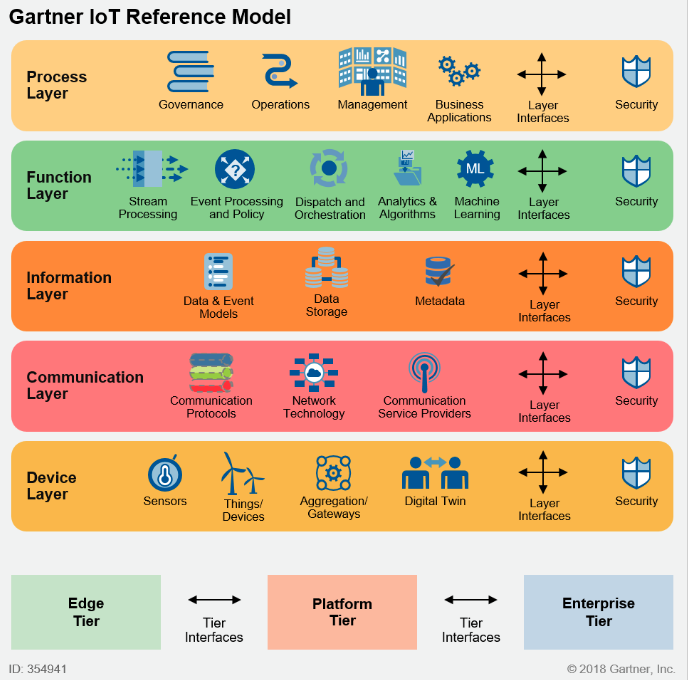
\includegraphics[width=100mm,scale=1]{Figures/gartnerIoT}
	\decoRule
	\caption[Gartner]{Gartner Layer Model}
	\label{fig:gartnerIoT}
\end{figure}



\subsection{Five-Layer architecture}
One by \parencite{fiveLayer1,fiveLayer} proposed model is a five-layer-model consisting of the following layers.
\begin{description}
    \item [Perception layer] \hfill \\
    The perception layer is the physical layer of the architecture. Sensors and actuators exist in this layer.
    \item [Transport layer] \hfill \\
     The transport layer transports data from the perception layer to the processing layer. Different network protocols can be used
   \item [Processing layer] \hfill \\
   The processing layer stores, analyzes and channels incoming data. It is also known as the middleware layer.
   \item [Application layer] \hfill \\
   The application layer is responsible for delivering user-relevant data to a user.
   \item [Business layer] \hfill \\
   The business layer manages the whole system, e.g. applications, business and profit models.
\end{description}


When talking about IoT-architectures, one should mention the difference between cloud and fog/edge based architectures. 

Cloud based architectures assume that processing and analyzing of data should happen in an enviroment remote from the devices' location.
The network below sends data to the cloud, and above the cloud lie applications working with the processed data with the cloud in the center of this architecture.
In the last years, cloud computing has gained popularity, also in the context of IoT architectures \parencite{CloudComputing} because it provides great exibility and scalability.

A newer trend instead are fog or edge based architectures, where the sensors and gateways do parts of the data processing and analytics.
A fog architecture \parencite{FogComputing1, FogComp} presents a layered approach, inserting various layers between the physical (perception) and transport layers 
(monitoring, pre-processing, storage, security). 
Wheras fog computing refers to smart sensors and gateways, edge computing refers to not-smart objects like motors, pumps with 
smart data preprocessing capabilities \parencite{edgeFog}.


\section{Front-End}
As \parencite{frontendDef} states:
"A front-end system is part of an information system that is directly accessed and interacted with by the user to receive or 
utilize back-end capabilities of the host system. 
It enables users to access and request the features and services of the underlying information system."  

The front-end is the visual component of any application. 

Disciplines like UX (User Experience), UI(User Interface) and  IxD (Interaction design) have been working on creating 
a "better" front-end-experience for many years. 

Usually, a mixture of HTML, CSS and Javascript is used for front-end development. 
In recent years, libaries that combine HTML and Javascript capabilities like React.js, Angular or Vue %\parencite{reactjsAngularVue} 
have been designed to support a component based architecture. 

For this project, React.js was used. React.js will further be called by it's commonly referred name "React".
React is an Open-Source Javascript-Libary.
After developing React in 2011, Facebook soon discovered that it's performance was faster than other implementations of its' kind \parencite{benchmarkReact}and made it Open-Source in 2015. 
At present, React is used by major companies for their front-end like Airbnb, Netflix and Reddit \parencite{reactjsUsers}. 
In this years' Stackoverflow-Survey, React came third in "Most Popular Framework, Libary or Tool" \parencite{stackOverflowSurvey}. 
This year, over 100,000 developers participated in the survey. 
A lot of libaries are available for React. 
Its main concepts are:


\begin{description}
    \item[Components] \hfill \\
    React motivates its users to write encapsulated components with single responsibilities. Components combine the HTML-markup and Javscript-functionality of a responsibility. 
    They are supposed to increase reusability. %erhöhen
    \item[Composition] \hfill \\
    The user can reuse and composite elements as he needs to. 
    The isolated components make code easier to maintain. 
    \item[Uni-Directional Dataflow] \hfill \\
            Properties should not be changed in other components, but passed down as read-only variables. 
            React doesn't want children to affect their parent components. That makes maintainability easier, as there's a clear downward structure in a well designed React project.
            If a user needs to pass changes to a parent component, it's executed with callbacks.
    \item[Virtual Dom]\hfill \\
    A Document Object Model (DOM) is a logical structure of documents in HTML, XHTML, or XML formats. 
    Web browsers are using layout engines to transform or parse the representation HTML-syntax into document object model that we can see in a web browser.
    Usually, when one of these elements changes, the whole structure has to be calculated again. 
    React uses a Virtual DOM as a negiator to enable calculating only the parts that need calculating. That's also possible because of Reacts' isolated component structure.
    \item[JSX] \hfill \\
    %ÜBERARBEITEN
    //ÜBERARBEITEN 

    Javascript XML (JSX), is a Javascript extension of Javascript which is usually used to write in ReactJs. 
    It looks a lot like HTML but enables Javascript functionality. 
    Javascript functionalities can be used by putting them in curly brackets ("{}").
\end{description}
\begin{figure}[b]
	\centering
    \includegraphics[width=125mm, scale=1.25]{Figures/ReactExampleFullsize}
	\decoRule
	\caption[React1]{React example code}
	\label{fig:reactEx}
\end{figure}

\begin{figure}[t]
    \centering
	\includegraphics[width=75mm,scale=0.75]{Figures/EditExample1}
	\decoRule
	\caption[ReactEx]{Resulting Output of example code}
	\label{fig:resultReact}
\end{figure}


\section{Communication}
%Socket.io
There are different ways to communicate between clients and middleware. 
Communication on the web is usually unsynchronized. 
That means that the client requests something and the server responds. 
Problems arise if real-time communication is required. 
Chat-applications e.g. shouldn't require the user to reload a page anytime he wants to see a new message.
Those services demand a more reactive and immediate communication.

For this, web development techniques like AJAX \parencite{ajax} were invented. 
Here, the client requests data automatically, establishing a new connection to the server.

This technique needs a client to request new content instead of listening 
for new information which creates unnessecary overhead and a higher latency than other communication enviroments like websockets.  
 
Websockets pursue this task by creating a bilateral environment for clint-server-exchange. 
This way, the client doesn't need to connect again and again, but listens for events. 
Now-a-days, most browsers are websocket compatible.

For this project, Socket.io was used for client-middleware-communication.

Socket.io is a Javascript-Libary designed for realtime communication build on top of a websocket-protocol.
It enables a bi-directional communication channel between client and server and offers a fallback mechanism to long polling when websockets are not available.
There are several fallback mechanisms available that are determined dynamically by Socket.io:
\begin{itemize}
    \item Websocket
    \item Adobe Flash Socket
    \item AJAX long polling
    \item AJAX multipart streaming
    \item Forever Iframe
    \item JSONP Polling
\end{itemize}

The server-side of Socket.io is developed  specifically for Node.js wheras for the client different implementations (e.g. .Net, Swift, C++)\parencite{socketioClients} are available.
Once a connections is established it's maintained and uses a diminishing small amount resources to communicate. 
It uses an event-based system where one participant listens and another emits an event. 
Both Client and Server can emit and listen for events.

\section{Middleware}
%Talk about Node.js
Middleware is "software that acts as a bridge between an operating system or database 
and applications, 
especially on a network" \parencite{middlewaredef}. 

As happening in other contexts, 
a Service Orientated Architecture (SOA) approach for middleware 
was proposed in many IoT - architectures from the last few years \parencite{archsurv1}. 
SOA encourages decomposition of a complex system into simpler and isolated components.
Thus, reusability and changeability is increased. 
Especially an IoT-scenario with flexible gateway components and on-going extensions can profit from such 
architecture as changes are demanded frequently.

\parencite{archsurv1}
In this case, Node.js was used as middleware between our client front-end and the database-backend.

Node.js is an open-source, cross-plattform, javascript-runtime-enviroment. 
With 49.6\% it is this years "Most Popular Framework, Libary or Tool" on this years Stackoverflow-survey \parencite{stackOverflowSurvey}.
According to Google Trends, interest is rising since 2012\parencite{gogleTrendNode}.
One explanation for that might be that it's written in Javascript. 
The transition for front-end Javascript developers to developing back-end is eased, which saves companies learning costs \parencite{nodejssavescost}.
It uses an event-driven architecture which operates on a single threaded event loop using non-blocking I/O calls.
Commands use callbacks to signal they are completed or failed. 
A downside is, that it doesn't allow vertical scaling by increasing the number of CPU cores of the machine it is running on. 
On CPU-intensive applications, that might become a problem - but modules like IPC or pm2 can add that functionality.
Node.js commands are non-blocking and execute concurrently or in parallel. 
It's build on the Google V8 JavaScript engine which compiles Javascript to machine code instead of interpreting it in real time. 
%Statistik zu schnelligkeit
There are thousands of open-source libaries and web frameworks available for Node.js. 

\section{Device}
%Talk about Arduino implementation
An IoT-Device can take many forms: 
Sensors and actuators can be used to create nearly any use case, 
from motion detection for light automation, to tracking the productivity of a machine to automated heating depending on room temperature.

\subsection{Arduino}
A popular choice for self-made technology projects is the Arduino microprocessor.

Arduino is a microcontroller-company from italy which was founded in 2005. 
It is completely open source and provides its own Integrated Development Enviroment(IDE) \parencite{arduinoIDEDownload}.
The IDE works with nearly all microprocessors on the market. 
The IDE recommends a structure for all Arduino programs:
\begin{description}
    \item [Initialization]
    Prior to any function, libaries and necessary variables are declared within an Arduino program.
    \item [setup()]
    The setup-function is the first function called in any Arduino-program. 
    This is were variables, supporting hardware or the serialport are initialized and pin modes are set. 
    \item [loop()]
    The loop-function loops consecutively, 
    which enables the program to change and respond on run-time.
    Checking for changes usually happens here, 
    whereas consequences of those changes are implemented outside the loop-function.    
\end{description}
The Arduino (and comperable microprocessors) are programmed in C.

Right now, the Arduino is not the most typical choice for IoT-devices in particular as Arduinos 
with included supporting hardware (e.g. Wi-Fi-modules) released just this year,
however due to it's popularity many libaries and instructions exist to introduce an Arduino to an IoT-scope.
E.g. with additional hardware like a Wi-Fi shield and existing free apps like "Blynk"  \parencite{blynk}, 
an Arduino can be tracked and controlled within 30 minutes of set-up.

\begin{figure*}[h]
	\centering
	\copyrightbox[r]{\includegraphics[width=75mm,scale=0.75]{Figures/adafruitSPI}}{\textcopyright https://learn.sparkfun.com/tutorials/serial-peripheral-interface-spi/all }
	\caption{Visualization of SPI communication}
  \end{figure*}



\section{Back-End}
%Talk about postgres
According to the Oxford Dictionary, a back-end is 
"The part of a computer system, piece of software, etc., where data is stored or processed rather 
than the parts that are seen and directly used by the user" \parencite{backendDef}

If an architecture contains middleware, the back-end is usually responsible for storing and retrieving data for other parts of the system.
Accordingly, a database and a database management system (DBMS) are introduced.
The database stores the data, whereas the DBMS makes the data accessable from elsewhere.
Famous, established examples for DBMS are MySQL and Oracle.
Most DBMS are heavily influenced by the standardised SQL-language which was first introduced in 1970 by Edgar F. Codd in context with the relational model.
An important idea of the relational model is the concept of database normalization, where related records are linked by a key predicate common to all.

For this database, PostgreSQL was used.
PostgreSQL is a light-weight open-source object-relational database system. 
Companies like Netflix, Spotify or Instagram \parencite{postgresUsers} rely on the flexible database system which allows SQl and noSQL design.
It is easy to set-up and maintain. 


%Even though, only 26\% of IoT-Projects in companies are judged to be a complete success 
%\parencite{ciscoresearch}. The reasons are as numerous as they are diverse. 
%Lack of knowledge, lack of planning, inconsistent standards and legacy architectures within the project are only some mentioned by the Cisco survey.
%A McKinsey report \parencite{mcKinsey} in 2015 stated that most IoT adopters fail to use their data or derive just a small part of its value.
